
\section{Is every individual happy after equilibrium?} 
\label{sec:meanhappy}
As shown in section \ref{sec:equi}, equilibrium is not always reached within 10000 generations, stronger even, equilibrium is occasionally never reached at all.
But when it does, it is natural to question whether every individual is happy and how happy they are. 
To answer this question, we ran 500 simulations for each HR ranging from 0 to 1 with increments of $0.01$ and we calculated the average, maximal and minimal happiness of the population for each happiness rule. 
We ran the simulations om the standard board and the results are shown in Figure \ref{happyhappy}.\\

From Figure \ref{happyhappy}, we observe that the minimal happiness is almost always equal to or greater than the happiness rule, which means that every individual is in fact happy  in the equilibrium. 
We also see that maximal happiness is always 1, which means there is always at least one invididual who lives homogenous. 
Furthermore, we see that the average happiness is always closer to the maximal happiness than to the minimal happiness. At a HR of approximately $0.8$, we see that every individual has happiness 1. 
This implies that happiness $0.8$ guarantees nearly full segregation. Complete segregation can only be assured at a HR greater than $0.875$, Namely, assume a person does not live in a homogenous neighbourhood, then at least 1 out of at most 8 neighbours does not share his/her type. In other words, the happiness of this person is at most equal to \(1-\frac{1}{8}=0.875\).\\

It is not very surprising that every individual is happy after the equilibrium, since it would otherwise mean that one individual is unable to find a place that better meets his/her desire, which seems rather unlikely on a board with $24$ empty spaces. 
Another remarkable result is that Figure \ref{happyhappy} shows that the minimal happiness is higher than the HR and that the average happiness is nearly 1 if the happiness rule higher than $0.8$. 
At first glance, this might seem impossible because the heavy requirement of being happy, but on the other hand, it shows that the strong 'need' for segregation actually leads to greater happiness.

\begin{figure}[h!]
    \centering
    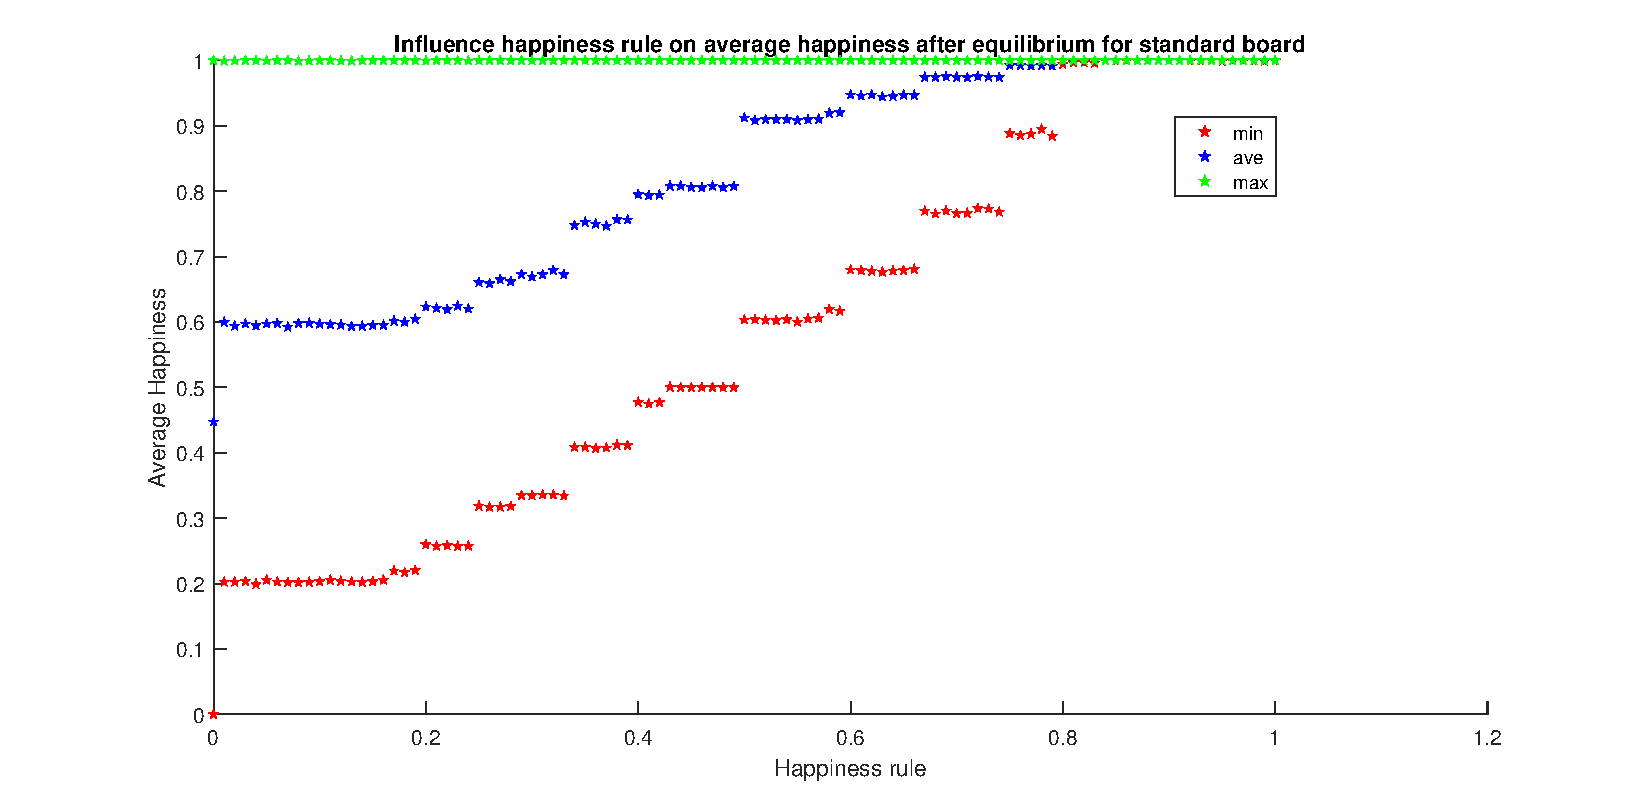
\includegraphics[width=0.9\textwidth]{happinessregel-gemhappinesseind-2.pdf}
    \caption{Effect of happiness rule on the happiness of the individuals. The green graph shows the maximal happiness, the blue graph shows the average happiness and the red graph shows the minimal happiness}
    \label{happyhappy}
\end{figure}

To illustrate that the variance of every above calculated average happiness is very low, we  selected Happiness Rule $1/3$ as an example and made a histogram in Figure \ref{minhappy}, showing that the probability that any individual is happy is practically $1$.

\begin{figure}[H]
    \centering
    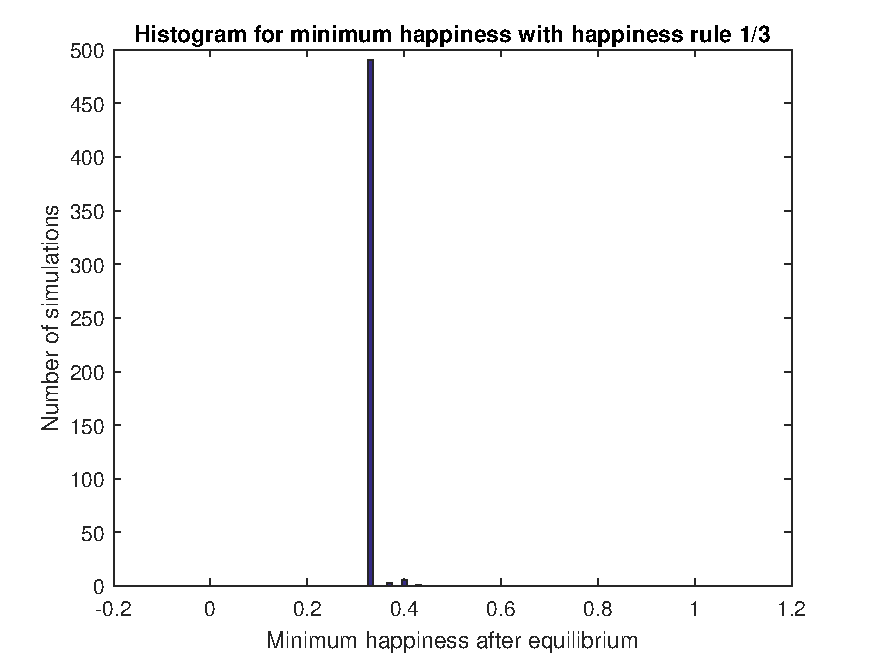
\includegraphics[width=0.9\textwidth]{histogram_min_happiness_een_derde.pdf}
    \caption{Histogram for minimum happiness after 500 simulations with HR=1/3 }
    \label{minhappy}
\end{figure}

%Ik plaats hier random text om ervoor te zorgen dat dingen goedgaan met invoegen gelieve aan te passen.
